\documentclass{article}

\usepackage{url}

\usepackage{amssymb,amsfonts,amsmath,amsthm,mathtools}
\usepackage{adjustbox}
\usepackage{float}
\usepackage{caption}
\usepackage{mdframed}
\usepackage{lmodern}
\usepackage{bm,bbold}
\usepackage{xfrac, nicefrac}
\usepackage{xcolor}
\usepackage{lmodern}
\usepackage{enumitem}
\usepackage{pgfplots, pgf,tikz}
\usepackage[margin=60pt]{geometry}
\pdfinclusioncopyfonts=1

\definecolor{RED}{HTML}{EB6231}
\definecolor{YELLOW}{HTML}{E29D26}
\definecolor{BLUE}{HTML}{5D80B4}
\definecolor{LIGHTGREEN}{HTML}{6ABD9B}
\definecolor{GREEN}{HTML}{8FB03E}
\definecolor{PURPLE}{HTML}{BE1E2D}
\definecolor{BROWN}{HTML}{A97C50}
\definecolor{PINK}{HTML}{DA1C5C}
\captionsetup{width=0.85\textwidth}

\newcommand{\specialcell}[2][c]{%
	\begin{tabular}[#1]{@{}c@{}}#2\end{tabular}}

\DeclareMathOperator{\E}{\mathbb{E}}
\newcommand{\der}{\mathrm{d}}
\newcommand{\e}{\mathrm{e}}

% Time, effective population size and mutation rate.
\newcommand{\Ne}{N_{\mathrm{e}}}
\newcommand{\dnds}{\omega}
\newcommand{\Nsite}{\text{n}}
\newcommand{\Nstate}{\text{K}}

\newcommand{\x}{x}
\newcommand{\eq}{^{*}}
\newcommand{\dx}{\delta \x}

\begin{document}
\part*{Supplementary materials}

\section*{Genotype to phenotype map}
Define $\Nsite$ as the number of sites in the genotype sequence.
Each site can be in one of $\Nstate \geq 2$ states, where only $1$ state is defined the stable state, and $\Nstate - 1$ states are unstable.
For a given genotype sequence, define phenotype $0 \leq \x \leq 1$ as the current proportion of sites in the unstable state.
After a mutation, given that only one site can change at a time, the absolute change of $\x$ is either $0$ or $\dx=\sfrac{1}{\Nsite}$.
Define $\rho_{\x}(\dx)$ as the probability to get a change of phenotype equal to $\dx$, if the current phenotype is $\x$:\\
\begin{gather}
\begin{cases}
\dx &\text{ with probability } \rho_{\x}(\dx) = 1-x, \\
0 &\text{ with probability } \rho_{\x}(0) = \x \left[1 - \frac{1}{\Nstate - 1}\right], \\
-\dx &\text{ with probability } \rho_{\x}(-\dx) = \frac{x}{\Nstate - 1}.\\
\end{cases} \label{eq:proba}
\end{gather}

\section*{Selection coefficient}
$s(\x, \dx)$ is the selection coefficient of an effect $\dx$ if the current phenotype is $\x$:
\begin{align}
s(\x, \dx) &= \frac{f(\x + \dx) - f(\x)}{f( \x)}, \\
 &\simeq \frac{1}{f(\x)}\frac{\der f( \x)}{\der \x} \dx, \\
 &\simeq \frac{\der \ln (f(\x))}{\der \x} \dx, \label{eq:s_from_fitness}
\end{align}
where $f( \x)$ is the Wrightian fitness of phenotype $x$. And thus we also have:
\begin{gather}
s(\x, -\dx) \simeq - s(\x, \dx) \text{ from eq. \ref{eq:s_from_fitness}} \label{eq:s_minus_deltax}, \\
\iff S(\x, -\dx) \simeq - S(\x, \dx), \label{eq:S_minus_deltax}
\end{gather}
where $S(\x\eq, \dx) = 4\Ne s (\x\eq, \dx)$ is the scaled selection coefficient.

\section*{Probability of fixation}
The probability of fixation of a mutation with effect $\dx$, for a resident phenotype $\x$ is :
\begin{align}
p_{\text{fix}}(\x, \dx) &= \frac{ 2 s(\x, \dx)}{1 - \e^{-4\Ne s(\x, \dx)}}, \\
 &= \frac{ 2 s(\x, \dx)}{1 - \e^{-S(\x, \dx)}}. \label{eq:pfix}
\end{align}
And in the case of neutral mutations, the probability of fixation is:
\begin{gather}
p_{\text{fix}}(\x, 0) = \frac{ 1}{2 \Ne} \label{eq:pfix0}.
\end{gather}
And the ratio of probability of fixation between selected and neutral mutations is:
\begin{align}
\frac{p_{\text{fix}}(\x, \dx)}{p_{\text{fix}}(\x, 0)} & = \frac{ 2 \Ne 2 s(\x, \dx)}{1 - \e^{-S(\x, \dx)}},\\
& = \frac{S(\x, \dx)}{1 - \e^{-S(\x, \dx)}} \label{eq:pfixratio}.
\end{align}
\section*{Equilibrium phenotype}
At equilibrium phenotype $\x\eq$, the expected selection coefficient of mutation that reached fixation must be $0$:
\begin{gather}
 0 = \E_{\dx} \left[ s(\x\eq, \dx) p_{\text{fix}}(\x\eq, \dx) \right], \\
\iff 0 = \E_{\dx} \left[ s(\x\eq, \dx)\frac{ 2 s(\x\eq, \dx)}{1 - \e^{-S(\x\eq, \dx)}} \right], \\
\iff 0 = s(\x\eq, \dx)\frac{ 2s(\x\eq, \dx)}{1 - \e^{-S(\x\eq, \dx)}}   \rho_{\x\eq}(\dx) + s(\x\eq, 0) \frac{ \rho_{\x\eq}(0)}{2\Ne} + s(\x\eq, -\dx)\frac{ 2s(\x\eq, -\dx)}{1 - \e^{-S(\x\eq, -\dx)}}   \rho_{\x\eq}(-\dx), \\
\Longrightarrow s(\x\eq, \dx) \frac{ 2s(\x\eq, \dx)}{1 - \e^{-S(\x\eq, \dx)}}   \rho_{\x\eq}(\dx) \simeq s(\x\eq, \dx) \frac{ - 2s(\x\eq, \dx)}{1 - \e^{S(\x\eq, \dx)}}   \rho_{\x\eq}(-\dx) \text{ from eq. \ref{eq:S_minus_deltax}}, \\
\iff \frac{ \rho_{\x\eq}(\dx)}{\rho_{\x\eq}(-\dx)} \simeq \e^{-S(\x\eq, \dx)} \frac{ \e^{-S(\x\eq, \dx)} - 1}{ \e^{-S(\x\eq, \dx)} \left( 1 - \e^{S(\x\eq, \dx)} \right)}, \\
\iff \ln \left( \frac{1 - \x\eq}{\x\eq} \right) + \ln (\Nstate-1) \simeq -S(\x\eq, \dx) \text{ from eq. \ref{eq:proba}} \label{eq:equilibrium}, \\
\iff \x\eq \simeq \frac{1}{1 + \frac{\e^{-S(\x\eq, \dx)}}{\Nstate-1}}.
\end{gather}

\section*{Substitution rate ($\bm{\dnds}$)}
The substitution rate of selected mutations relative to neutral mutations  ($\dnds$) is by definition:
\begin{align}
\dnds & = \E_{\dx} \left[ \frac{p_{\text{fix}}(\x, \dx)}{p_{\text{fix}}(\x, 0)} \right], \\
 & = \E_{\dx} \left[ \frac{ S(\x, \dx)}{1 - \e^{-S(\x, \dx)}} \right], \\
 & = (1 - \x) \frac{ S(\x, \dx)}{1 - \e^{-S(\x, \dx)}} + \x \left(\frac{\Nstate - 2}{\Nstate - 1}\right) + \frac{\x}{\Nstate-1} \frac{ S(\x, -\dx)}{1 - \e^{-S(\x, -\dx)}} \text{ from eq. \ref{eq:proba}}, \\
 & = (1 - \x) \frac{ S(\x, \dx)}{1 - \e^{-S(\x, \dx)}} - \frac{\x}{\Nstate-1}  \frac{ S(\x, \dx)}{1 - \e^{S(\x, \dx)}} +  \x \left(\frac{\Nstate - 2}{\Nstate - 1}\right) \text{ from eq. \ref{eq:S_minus_deltax}}.
\end{align}
$\dnds\eq$ at equilibrium is then determined by the phenotype at equilibrium $\x\eq$:
\begin{align}
\dnds\eq &= (1 - \x\eq) \frac{ S(\x\eq, \dx)}{1 - \e^{-S(\x\eq, \dx)}} - \frac{\x\eq}{\Nstate-1} \frac{ S(\x\eq, \dx)}{1 - \e^{S(\x\eq, \dx)}} + \x\eq \left(\frac{\Nstate - 2}{\Nstate - 1}\right) , \\
 &= \x\eq \left[ \frac{2 (\x\eq-1)  \left(\ln (\Nstate-1)+\ln \left(\frac{1 -\x\eq}{\x\eq}\right)\right)}{\Nstate (\x\eq-1)+1} + \frac{\Nstate - 2}{\Nstate - 1}\right] \text{ from eq. \ref{eq:equilibrium}}.
\end{align}
\begin{center}
	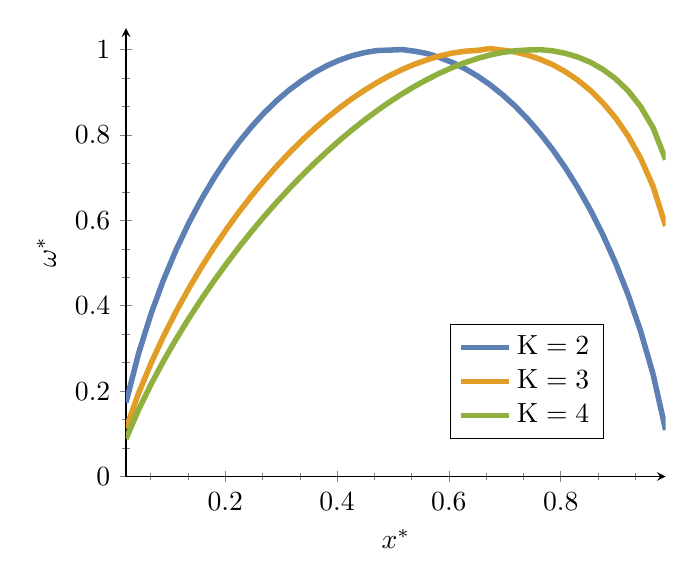
\begin{tikzpicture}
	\begin{axis}[
	ylabel={$\dnds\eq$},
	xlabel={$\x\eq$},
	domain=0:1.1,
	ymin=0.0, ymax=1.05,
	samples=50,
	legend entries={$\Nstate=2$, $\Nstate=3$, $\Nstate=4$},
	legend cell align=left,
	minor tick num=2,
	axis x line=bottom,
	axis y line=left,
	legend style={at={(0.6,0.34)},anchor=north west}
	]
	\addplot[line width=2.0pt, color=BLUE]{ (ln(2-1) + ln((1-x) / x)) * x * 2 * (x - 1) / (2 * (x - 1) + 1) + x * (2-2) / (2-1) };
	\addplot[line width=2.0pt, color=YELLOW]{ (ln(3-1) + ln((1-x) / x)) * x * 2 * (x - 1) / (3 * (x - 1) + 1) + x * (3-2) / (3-1)};
	\addplot[line width=2.0pt, color=GREEN]{ (ln(4-1) + ln((1-x) / x)) * x * 2 * (x - 1) / (4 * (x - 1) + 1) + x * (4-2) / (4-1)};
	\end{axis}
	\end{tikzpicture}
\end{center}
And the derivative of $\dnds\eq$ w.r.t to $\x\eq$ is: 
\begin{gather}
\frac{\der \dnds\eq}{\der \x\eq} = 2 \left[ \frac{\Nstate (\x\eq- 1) + 1+\left[\Nstate (\x\eq-1)^2+2 \x\eq-1\right] \left[ \ln (\Nstate-1) + \ln \left(\frac{1 - \x\eq}{\x\eq} \right) \right]}{(\Nstate (\x\eq-1)+1)^2}\right] + \frac{\Nstate - 2}{\Nstate - 1} \label{eq:dw_dx}.
\end{gather}

\begin{center}
	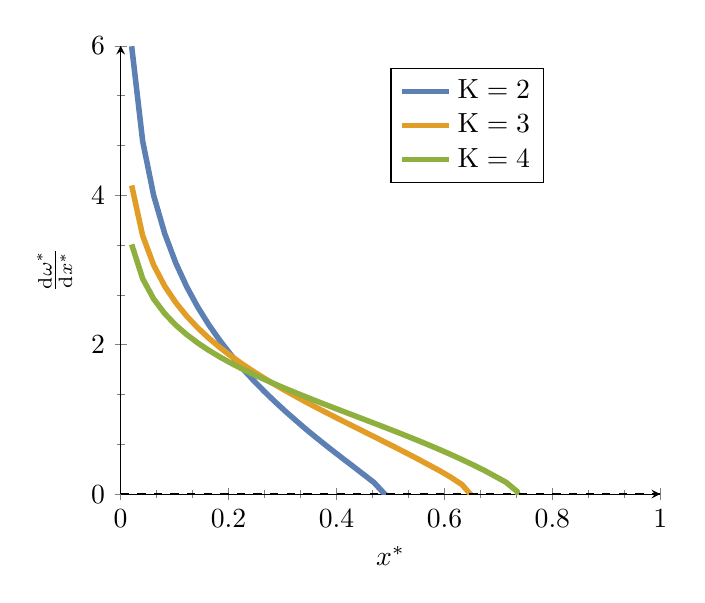
\begin{tikzpicture}
	\begin{axis}[
	ylabel={$\frac{\der \dnds\eq}{\der \x\eq}$},
	xlabel={$\x\eq$},
	domain=0.0:1.0,
	ymin=0, ymax=6,
	samples=50,
	legend entries={$\Nstate=2$, $\Nstate=3$, $\Nstate=4$},
	legend cell align=left,
	minor tick num=2,
	axis x line=bottom,
	axis y line=left,
	legend style={at={(0.5,0.95)},anchor=north west}
	]
	\addplot[line width=2.0pt, color=BLUE]{2*(2*(x-1)+1 + (2*(x-1)^2+2*x-1)*(ln(2-1) + ln((1-x)/x)))/(2*(x - 1) + 1)^2 + (2-2) / (2-1) };
	\addplot[line width=2.0pt, color=YELLOW]{2*(3*(x-1)+1 + (3*(x-1)^2+2*x-1)*(ln(3-1) + ln((1-x)/x)))/(3*(x - 1) + 1)^2 + (3-2) / (3-1) };
	\addplot[line width=2.0pt, color=GREEN]{2*(4*(x-1)+1 + (4*(x-1)^2+2*x-1)*(ln(4-1) + ln((1-x)/x)))/(4*(x - 1) + 1)^2 + (4-2) / (4-1)};
	\addplot[dashed,line width=0.5pt, color=black]{0};
	\end{axis}
	\end{tikzpicture}
\end{center}

\section*{Substitution rate ($\bm{\dnds}$) for the special case \Nstate=2}
In the special of $2$ states ($1$ stable and $1$ unstable), $\dnds\eq$ at equilibrium is:
\begin{align}
\dnds\eq & = \ln \left( \frac{1 - \x\eq}{\x\eq} \right) \frac{2 (\x\eq -1) \x\eq }{2 \x\eq - 1},\\
& = \begin{cases}
 - 2 \x\eq \ln (\x\eq) + \mathcal{O}({\x\eq}^2) \text{ as } \x\eq \rightarrow 0, \\
 1 - \frac{8}{3} (\x\eq - 0.5)^2 + \mathcal{O}((\x\eq - 0.5)^3) \text{ as } \x\eq \rightarrow 0.5. \\
\end{cases}
\end{align}
\begin{center}
	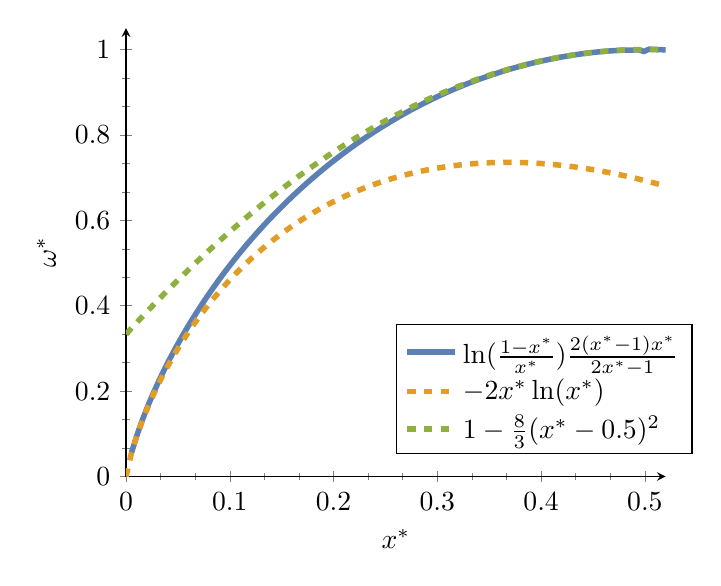
\begin{tikzpicture}
	\begin{axis}[
	ylabel={$\dnds\eq$},
	xlabel={$\x\eq$},
	domain=0:0.52,
	ymin=0.0, ymax=1.05,
	samples=100,
	legend entries={
		$\ln( \frac{1 - \x\eq}{\x\eq}) \frac{2 (\x\eq -1) \x\eq }{2 \x\eq - 1}$,
		$- 2 \x\eq \ln (\x\eq)$,
		$ 1 - \frac{8}{3} (\x\eq - 0.5)^2$},
	legend cell align=left,
	minor tick num=2,
	axis x line=bottom,
	axis y line=left,
	legend style={at={(0.5,0.34)},anchor=north west}
	]
	\addplot[line width=2.0pt, color=BLUE]{ ln((1-x) / x) * x * 2 * (x - 1) / (2 * x - 1)};
	\addplot[dashed,line width=2.0pt, color=YELLOW]{ -2 * x * ln(x) };
	\addplot[dashed,line width=2.0pt, color=GREEN]{ 1 - 8 * (x - 0.5)^2 / 3 };
	\end{axis}
	\end{tikzpicture}
\end{center}
And the derivative of $\dnds\eq$ w.r.t to $\x\eq$ is: 
\begin{align}
\frac{\der \dnds\eq}{\der \x\eq} &= \frac{\ln \left( \frac{1 - \x\eq}{\x\eq} \right)(2 - 4 \x\eq + 4 {\x\eq}^2) + 4\x\eq - 2}{(2\x\eq -1)^2} \label{eq:dw_dx_Nstate2}, \\
&= 
\begin{cases}
 - (\x\eq + 1)(2\ln(\x\eq) + 2) - 2\x\eq + \mathcal{O}({\x\eq}^2) \text{ as } \x\eq \rightarrow 0, \\
 \frac{8 - 16 \x\eq}{3} + \mathcal{O}((\x\eq - 0.5)^2) \text{ as } \x\eq \rightarrow 0.5.
\end{cases} \label{eq:dw_dx_approx_Nstate2}
\end{align}

\begin{center}
	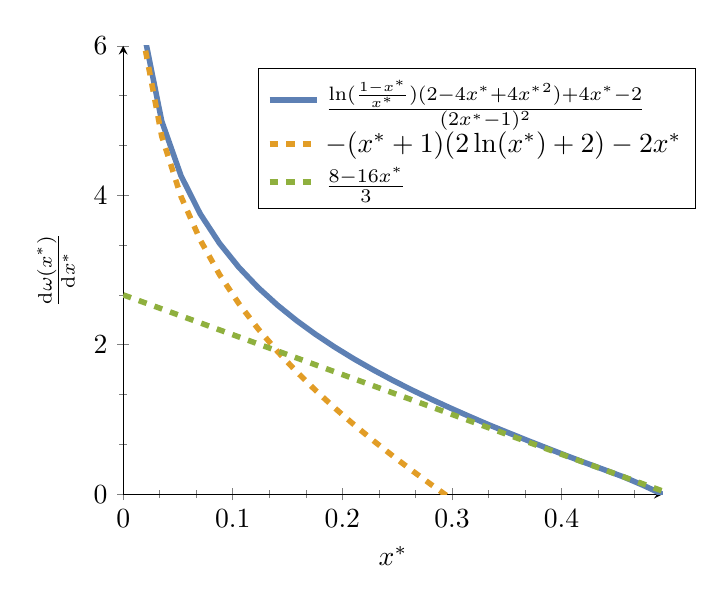
\begin{tikzpicture}
	\begin{axis}[
	ylabel={$\frac{\der \dnds(\x\eq)}{\der \x\eq}$},
	xlabel={$\x\eq$},
	domain=0.0:0.51,
	ymin=0.0, ymax=6,
	samples=30,
	legend entries={
		$\frac{\ln ( \frac{1 - \x\eq}{\x\eq})(2 - 4 \x\eq + 4 {\x\eq}^2) + 4\x\eq - 2}{(2\x\eq -1)^2}$,
		$- (\x\eq + 1)(2\ln(\x\eq) + 2) - 2\x\eq$,
		$\frac{8 - 16 \x\eq}{3}$},
	legend cell align=left,
	minor tick num=2,
	axis x line=bottom,
	axis y line=left,
	legend style={at={(0.25,0.95)},anchor=north west}
	]
	\addplot[line width=2.0pt, color=BLUE]{ (-2 + 4 * x + (2 - 4 * x + 4 * x^2) * ln((1-x) / x))/(1 - 2 * x)^2 };
	\addplot[dashed,line width=2.0pt, color=YELLOW]{ -(x+1)*(2*ln(x) + 2) -2*x };
	\addplot[dashed,line width=2.0pt, color=GREEN]{ 8 * ( 1 - 2*x)/3};
	\end{axis}
	\end{tikzpicture}
\end{center}

\section*{Change of equilibrium phenotype ($\bm{\x\eq}$) after a change in $\bm{\Ne}$}
Given the equilibrium equation (eq. \ref{eq:equilibrium}), $\x\eq$ is implicitly a function of $\Ne$, and the change of phenotype at equilibrium ($\der \x\eq$) after a change of effective population size ($\der \Ne$) can be obtain as:
\begin{gather}
G(\x, \Ne ) \equiv \ln \left( \frac{1 - \x}{\x} \right) + \ln (\Nstate-1) + 4 \Ne s(\x, \dx), \\
\iff G(\x\eq(\Ne), \Ne ) = 0 \text{ from eq. \ref{eq:equilibrium}}, \\
\Longrightarrow \frac{\partial G(\x\eq, \Ne ) }{\partial \x\eq }\frac{ \der \x\eq}{\der \Ne} + \frac{ \partial G(\x\eq, \Ne )}{\partial \Ne} = 0, \\
\iff \left[ \frac{\partial \ln (1-\x\eq) }{\partial \x\eq } - \frac{\partial \ln (\x\eq) }{\partial \x\eq}  + 4 \Ne \frac{ \partial s(\x\eq, \dx) }{\partial \x\eq } \right]\frac{ \der \x\eq}{\der \Ne} + 4 s(\x\eq, \dx) = 0, \\
\iff \left[ \frac{1}{(1 - \x\eq) \x\eq} + 4 \Ne \frac{ \partial^2 \ln f(\x\eq) }{\partial {\x\eq}^2}\dx \right]\frac{ \der \x\eq}{\der \Ne}  = - 4 \frac{ \partial \ln f(\x\eq) }{\partial {\x\eq}}\dx \text{ from eq. \ref{eq:s_from_fitness}}, \\
\iff 4 \dx \left[ \frac{1}{4 \dx \Ne  (1 - \x\eq) \x\eq} + \frac{ \partial^2 \ln f(\x\eq) }{\partial {\x\eq}^2} \right] \Ne \frac{ \der \x\eq}{\der \Ne}  = - 4 \dx \frac{ \partial \ln f(\x\eq) }{\partial {\x\eq}}, \\
\iff \frac{ \der \x\eq}{\der \ln (\Ne)}  = - \frac{\frac{ \partial \ln f(\x\eq) }{\partial {\x\eq}}}{\frac{1}{4 \dx \Ne  (1 - \x\eq) \x\eq} + \frac{ \partial^2 \ln f(\x\eq) }{\partial {\x\eq}^2}}  \label{eq:dx_dlnNe}.
\end{gather}
\section*{Change of equilibrium substitution rate ($\bm{\dnds\eq}$) after a change in $\bm{\Ne}$}
Together, the change of substitution rate at equilibrium ($\der \dnds\eq$) after a change of effective population size ($\der \Ne$) can be obtain as:
\begin{align}
\frac{\der \dnds\eq}{\der \ln (\Ne)} & = \frac{\der \dnds\eq}{\der \x\eq} \frac{ \der \x\eq}{\der \ln (\Ne)}, \\
 &= - \frac{\der \dnds\eq}{\der \x\eq} \frac{\frac{ \partial \ln f(\x\eq) }{\partial {\x\eq}}}{\frac{1}{4 \dx \Ne  (1 - \x\eq) \x\eq} + \frac{ \partial^2 \ln f(\x\eq) }{\partial {\x\eq}^2}} \text{ from eq. \ref{eq:dx_dlnNe}} \label{eq:dw_dlnNe}.
\end{align}
\section*{Phenotype to fitness mapping}
From a given phenotype $\x$, define the fitness as :
\begin{gather}
 f(\x) = \frac{1}{1 + \e^{\beta(\alpha + \kappa \x)}}, \label{eq:fitness}
\end{gather}
where $\alpha = \Delta G_0 < 0$ is the difference in free energy between stable and unstable protein when all sites are stable. $\kappa$ is the expected change in $\Delta G$ when all sites are unstable. By definition, $\kappa \dx = \sfrac{\kappa}{\Nsite} = \Delta \Delta G $\\
The derivative of fitness w.r.t to phenotype is:
\begin{align}
 \frac{\partial \ln (f(\x))}{\partial \x}  & = - \frac{\partial \ln \left( 1 + \e^{\beta(\alpha + \kappa \x)} \right)}{\partial \x} \text{ from eq. \ref{eq:fitness}}, \\
 & = - \beta \kappa \frac{\e^{\beta(\alpha + \kappa \x)}}{1 + \e^{\beta(\alpha + \kappa \x)}} \label{eq:df_dx}.
\end{align}
And the second derivative of fitness w.r.t to phenotype is:
\begin{align}
\frac{\partial^2 \ln (f(\x))}{\partial {\x}^2} & = - \beta \kappa \frac{\partial}{\partial \x} \left( \frac{\e^{\beta(\alpha + \kappa \x)}}{1 + \e^{\beta(\alpha + \kappa \x)}} \right) \text{ from eq. \ref{eq:df_dx}}, \\
 & = - \beta \kappa  \beta \kappa \frac{\e^{\beta(\alpha + \kappa \x)}}{\left( 1 + \e^{\beta(\alpha + \kappa \x)}\right)^2}, \\
 & = \frac{\beta \kappa}{1 + \e^{\beta(\alpha + \kappa \x)}} \frac{ \partial \ln f(\x) }{\partial {\x}} \text{ from eq. \ref{eq:df_dx}} \label{eq:df2_dx2}.
\end{align}
The equilibrium phenotype ($\x\eq$) is :
\begin{gather}
\ln \left( \frac{1 - \x\eq}{\x\eq} \right) + \ln (\Nstate-1) = 4\Ne \beta \kappa \frac{\e^{\beta(\alpha + \kappa \x\eq)}}{1 + \e^{\beta(\alpha + \kappa \x\eq)}}  \dx   \text{ from eq. \ref{eq:equilibrium} and \ref{eq:df_dx}}.
\end{gather}
Using $\Ne=10^4$, $\beta=1.686$, $\alpha = -118$, $\Nsite=300$, $\kappa=300$, we have the following:
\begin{center}
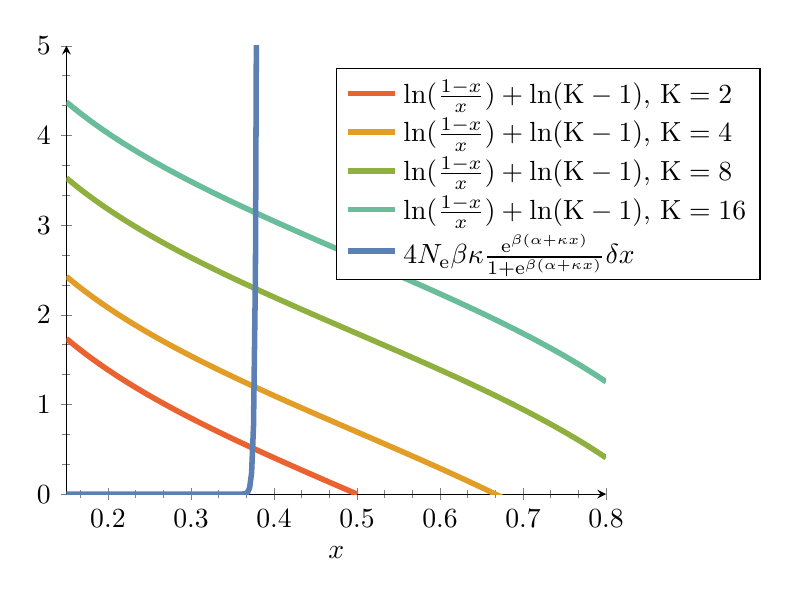
\begin{tikzpicture}
	\begin{axis}[
	xlabel={$\x$},
	ymin=0.0, ymax=5.0,
	samples=100,
	legend entries={
		$\ln(\frac{1 - \x}{\x}) + \ln(\Nstate-1) \text{, }\Nstate=2$,
		$\ln ( \frac{1 - \x}{\x})+ \ln(\Nstate-1) \text{, }\Nstate=4$,
		$\ln ( \frac{1 - \x}{\x})+ \ln(\Nstate-1) \text{, }\Nstate=8$,
		$\ln ( \frac{1 - \x}{\x})+ \ln(\Nstate-1) \text{, }\Nstate=16$,
		$4\Ne \beta \kappa \frac{\e^{\beta(\alpha + \kappa \x)}}{1 + \e^{\beta(\alpha + \kappa \x)}} \dx$},
	legend cell align=left,
	minor tick num=2,
	axis x line=bottom,
	axis y line=left,
	legend style={at={(0.5,0.95)},anchor=north west}
	]
	\addplot[domain=0.15:0.5,line width=2.0pt, color=RED]{ ln((1-x)/x) };
	\addplot[domain=0.15:0.68,line width=2.0pt, color=YELLOW]{ ln((1-x)/x) + ln(4-2) };
	\addplot[domain=0.15:0.8,line width=2.0pt, color=GREEN]{ ln((1-x)/x) + ln(8-2) };
	\addplot[domain=0.15:0.8,line width=2.0pt, color=LIGHTGREEN]{ ln((1-x)/x) + ln(16-2) };
	\addplot[domain=0.15:0.38, line width=2.0pt, color=BLUE]{ 4 * 1000 * 1.686 *exp(1.686 * (-118 + 300 *x))};
	\end{axis}
\end{tikzpicture}
\end{center}
\section*{Approximations}
We assume that $\Ne \gg 1$, $\alpha + \kappa \gg 1$ and $\kappa \dx \simeq 1$.
\begin{gather}
-S(\x\eq, \dx) \simeq 1, \\
\iff s(\x\eq, \dx) \simeq -\frac{1}{4 \Ne}, \\
\iff \frac{\der \ln (f(\x))}{\der \x} \simeq - \frac{1}{4 \Ne \dx}, \\
\iff \beta \kappa \frac{\e^{\beta(\alpha + \kappa \x)}}{1 + \e^{\beta(\alpha + \kappa \x)}} \simeq \frac{1}{4 \Ne \dx}, \\
\iff \frac{\e^{\beta(\alpha + \kappa \x)}}{1 + \e^{\beta(\alpha + \kappa \x)}} \simeq \frac{1}{4 \Ne \dx \beta \kappa}, \\
\Longrightarrow \frac{\e^{\beta(\alpha + \kappa \x)}}{1 + \e^{\beta(\alpha + \kappa \x)}} \ll 1, \\
\Longrightarrow \e^{\beta(\alpha + \kappa \x)} \ll 1, \\
\Longrightarrow \frac{\e^{\beta(\alpha + \kappa \x\eq)}}{1 + \e^{\beta(\alpha + \kappa \x\eq)}} \simeq \e^{\beta(\alpha + \kappa \x\eq)}.
\end{gather}
Moreover, we can get the following:
\begin{gather}
\frac{\der \ln (f(\x))}{\der \x} \simeq - \frac{1}{4 \Ne \dx}, \\
\iff \frac{ \partial^2 \ln f(\x) }{\partial {\x}^2} \simeq - \frac{1}{4 \Ne \dx \beta \kappa }, \\
\iff \frac{ \partial^2 \ln f(\x) }{\partial {\x}^2} \simeq - \frac{(1 - \x\eq)\x\eq }{\beta \kappa} \frac{1}{4 \dx \Ne  (1 - \x\eq) \x\eq}, \\
\Longrightarrow \frac{ \partial^2 \ln f(\x) }{\partial {\x}^2} \simeq - \dx \frac{(1 - \x\eq)\x\eq }{\beta } \frac{1}{4 \dx \Ne  (1 - \x\eq) \x\eq}, \\
\Longrightarrow \left| \frac{ \partial^2 \ln f(\x) }{\partial {\x}^2} \right| \gg \left| \frac{1}{4 \dx \Ne  (1 - \x\eq) \x\eq} \right|. \\
\end{gather}
Together, these approximations leads to:
\begin{align}
\frac{ \der \x\eq}{\der \ln (\Ne)} & = - \frac{\frac{ \partial \ln f(\x\eq) }{\partial {\x\eq}}}{\frac{1}{4 \dx \Ne  (1 - \x\eq) \x\eq} + \frac{ \partial^2 \ln f(\x\eq) }{\partial {\x\eq}^2}}, \\
& \simeq - \frac{\frac{ \partial \ln f(\x\eq) }{\partial {\x\eq}}}{\frac{ \partial^2 \ln f(\x\eq) }{\partial {\x\eq}^2}}, \\
& \simeq - \frac{1 + \e^{\beta(\alpha + \kappa \x\eq)}}{\beta \kappa}, \\
& \simeq - \frac{1}{\beta \kappa}.
\end{align}
Finally,
\begin{align}
\frac{ \der \dnds\eq}{\der \ln (\Ne)}  & \simeq - \frac{ \der \dnds\eq}{\der \x\eq} \frac{1}{\beta \kappa}, \\
  & = - \frac{1}{\beta \kappa}.
\end{align}
\section*{Numerical results}
\begin{center}
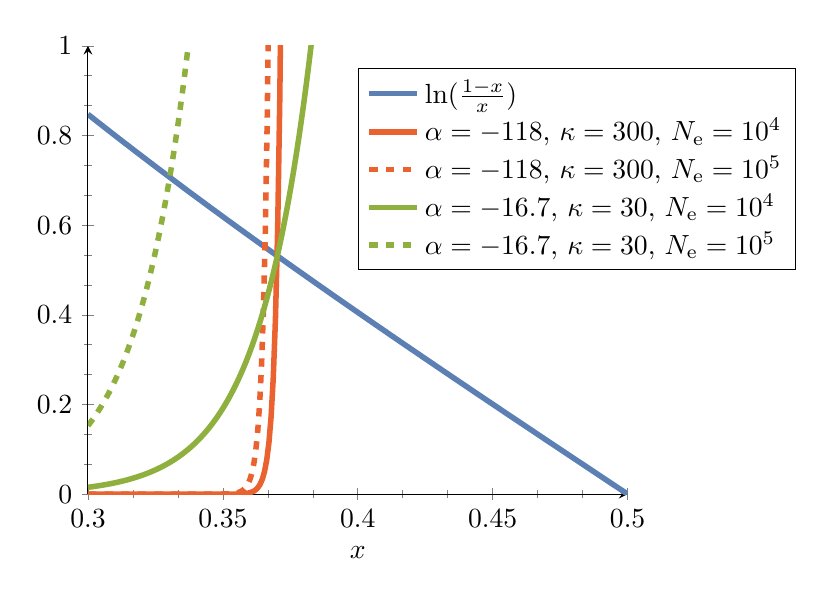
\begin{tikzpicture}
	\begin{axis}[
	xlabel={$\x$},
	ymin=0.0, ymax=1.0,
	samples=100,
	legend entries={$\ln(\frac{1 - \x}{\x})$,
		$\alpha = -118\text{, }\kappa = 300\text{, }\Ne = 10^{4}$,
		$\alpha = -118\text{, }\kappa = 300\text{, }\Ne = 10^{5}$,
		$\alpha = -16.7\text{, }\kappa = 30\text{, }\Ne = 10^{4}$,
		$\alpha = -16.7\text{, }\kappa = 30\text{, }\Ne = 10^{5}$},
	legend cell align=left,
	minor tick num=2,
	axis x line=bottom,
	axis y line=left,
	legend style={at={(0.5,0.95)},anchor=north west}
	]
	\addplot[domain=0.3:0.6,line width=2.0pt, color=BLUE]{ ln((1-x)/x) };		\addplot[domain=0.3:0.38, line width=2.0pt, color=RED]{4*10000*1.686*exp(1.686*(-118+300*x))};
	\addplot[dashed,domain=0.3:0.37, line width=2.0pt, color=RED]{4*100000*1.686*exp(1.686*(-118+300*x))};
	\addplot[domain=0.3:0.39, line width=2.0pt, color=GREEN]{4*10000*0.1*1.686*exp(1.686*(-16.71+30*x))};
	\addplot[dashed,domain=0.3:0.35, line width=2.0pt, color=GREEN]{4*100000*0.1*1.686*exp(1.686*(-16.71+30*x))};
	\end{axis}
\end{tikzpicture}
\end{center}
\end{document}